\documentclass[tikz]{standalone}
\usepackage{amsmath}
\begin{document}
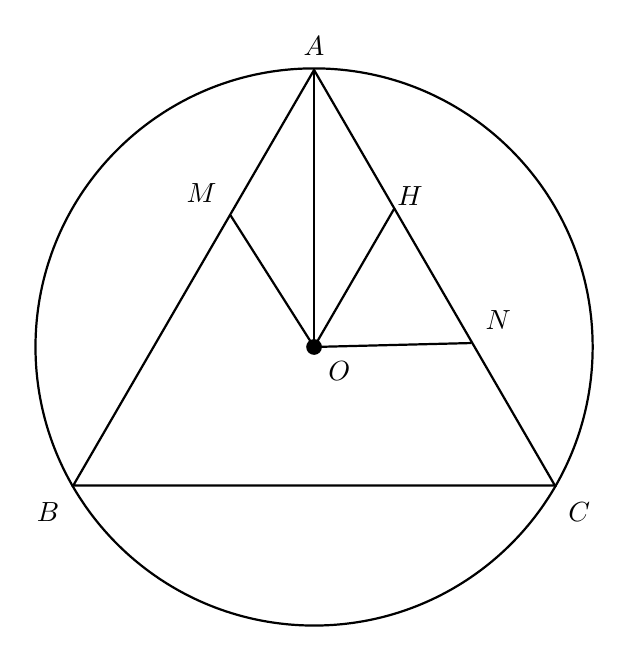
\begin{tikzpicture}[x=0.01cm, y=-0.01cm, line width=0.8pt]
  % 外接圆（圆心 O，半径 354）
  \draw (368,410) circle (354);

  % 三角形及辅助线
  \draw (368,58) -- (62,586) -- (674,586) -- cycle;
  \draw (368,58) -- (368,410);
  \draw (262,243) -- (368,410);
  \draw (368,410) -- (568,405);

  % 新增：OH 为过 O 且平行于 AB 的直线与 AC 的交点段（实线）
  \draw (368,410) -- (470,234);

  % 圆心点
  \fill (368,410) circle (0.1cm);

  % 标签
  \node at (368,28) {$A$};
  \node at (225,215) {$M$};
  \node at (30,620) {$B$};
  \node at (705,620) {$C$};
  \node at (602,376) {$N$};
  \node at (400,440) {$O$};
  \node at (490,218) {$H$};
\end{tikzpicture}
\end{document}
